%! TeX program = pdflatex
\documentclass{article}
\usepackage[english]{babel}
\usepackage[utf8]{inputenc}
\usepackage{amsmath}
\usepackage{amssymb}
\usepackage{minted}
\usepackage{listings}
\usepackage{xcolor}
\usepackage{algorithm}
\usepackage{algorithmicx}
\usepackage{hyperref}
\usepackage{graphicx}
% \usepackage{natbib}
\usepackage{subcaption} 
\usepackage{graphicx}
% \usepackage{url}
\usepackage{algorithm}% http://ctan.org/pkg/algorithms
\usepackage{algpseudocode}% http://ctan.org/pkg/algorithmicx
% \usepackage{tikz-cd}
\usepackage{listings}
\usepackage{xcolor}
% \usepackage[colorlinks, linkcolor = blue, citecolor = magenta]{hyperref}
\usepackage{float}
\usepackage{placeins}
\usepackage{pgfplots}
\usepackage{tikz}
\usepackage[margin=1in]{geometry}
\pgfplotsset{compat=1.18}
\usepackage{tikz}
\usetikzlibrary{positioning}
% % \usepackage{minted}
\usepackage{float}
% \usetikzlibrary{shapes, arrows, positioning}
% \lstset{ 
%     language=Python,                 % the language of the code
%     basicstyle=\ttfamily\small,      % the size of the fonts that are used for the code
%     numbers=left,                    % where to put the line-numbers
%     numberstyle=\tiny\color{gray},   % the style that is used for the line-numbers
%     stepnumber=1,                    % the step between two line-numbers. If it's 1, each line will be numbered
%     numbersep=5pt,                   % how far the line-numbers are from the code
%     backgroundcolor=\color{white},   % choose the background color. You must add \usepackage{color}
%     showspaces=false,                % show spaces adding particular underscores
%     showstringspaces=false,          % underline spaces within strings
%     showtabs=false,                  % show tabs within strings adding particular underscores
%     frame=single,                    % adds a frame around the code
%     rulecolor=\color{black},         % if not rolframe-color may be changed on line-breaks within not black text (e.g. comments (green here))
%     tabsize=4,                       % sets default tabsize to 4 spaces
%     captionpos=b,                    % sets the caption-position to bottom
%     breaklines=true,                 % sets automatic line breaking
%     breakatwhitespace=false,         % sets if automatic breaks should only happen at whitespace
%     title=\lstname,                  % show the filename of files included with \lstinputlisting; also try caption instead of title
%     keywordstyle=\color{blue},       % keyword style
%     commentstyle=\color{green},      % comment style
%     stringstyle=\color{red},         % string literal style
%     escapeinside={\%*}{*)},          % if you want to add LaTeX within your code
%     morekeywords={*,...} 
% }            % if you want to add more keywords to the rol\newenvironment{notation}
\newtheorem{remark}{Remark}
\newtheorem{definition}{Definition}
\newtheorem{property}{Property}
\newcommand{\DoParallel}[1]{\textbf{parallel do} \{#1\}}
\newcommand{\pder}[2]{\frac{\partial #1}{\partial #2}}

% Hyperref setup (often best loaded last, with exceptions like cleveref)
\hypersetup{
    colorlinks=true,
    linkcolor=blue,
    citecolor=magenta,
    urlcolor=cyan
}

\title{COLMENA Prototype for ANDES Power System Simulation}
\author{Pablo de Juan Vela $^{1}$ \\
        \small $^{1}$eRoots, Barcelona, Spain \\
}
\date{\today}

\usepackage[style=ieee, backend=biber]{biblatex}
\addbibresource{ref.bib}
\setlength{\parskip}{1em} 

\begin{document}
\maketitle

\section{Introduction}

This initial prototype showcases the main capabilities of COLMENA when applied to power system control problems. The prototype utilizes COLMENA's tools to react to grid disturbances and apply necessary corrective actions via predefined roles. The focus is on the roles themselves, how they respond to grid events, and how these responses improve the grid Key Performance Indicators (KPIs). This document provides an overview of the test grid, the roles and agents used in the simulation, and the specific mechanisms by which roles activate based on KPIs to modify the grid state. The prototype's code and implementation details are available in the Git repository \cite{git:eroots}.

\section{Grid Definition}

We chose a modified version of the IEEE 39-bus system \cite{grids:ieee39} as a testbed for the prototype. The original grid consists of 39 buses, 10 synchronous generators, and 19 loads. To better demonstrate COLMENA's capabilities, we replaced the synchronous generators with converters capable of operating in either Grid-Forming (GFM) or Grid-Following (GFL) mode. While there are several control options to choose from in a GFM converter, in this case, it will emulate the inertial behavior of a synchronous generator. The grid is modeled as a dynamic system evolving over time.
\begin{figure}[h]
    \centering
    \begin{center}
        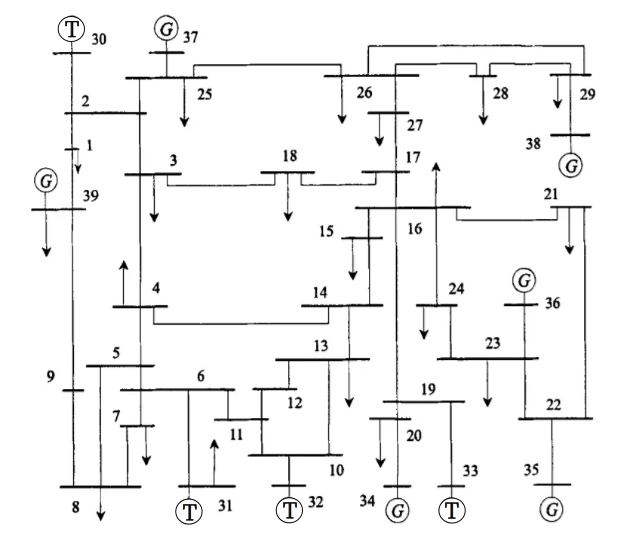
\includegraphics[width=0.8\textwidth]{plots/IEEE39withtrafo.png}
    \end{center}
    \caption{Modified IEEE 39-bus system topology used in the prototype, G mark generators and C the converters.}
    \label{fig:ieee39_topology}
\end{figure}

\subsection{Grid Dynamics}
Grid dynamics are influenced by several types of events:

\subsubsection*{Grid Topology Changes}
These changes directly affect the connection status of electrical devices, such as disconnecting a generator or experiencing a transmission line fault.

\subsubsection*{Device Mode Changes}
A change in operational mode alters the internal definitions and state variables of a device. Although power exchange at the connection bus might remain similar immediately following the change, the underlying control logic can be significantly different.

\subsubsection*{Device Set Point Changes}
In this case, the control logic itself remains unchanged, but reference values defining the desired steady-state operation are modified. For example, adjusting the reference voltage set point for a converter.

\section{Roles \& Agents}

\subsection{Agents}
The simulation involves six distinct agents. Three agents are coupled to converter devices, two are coupled to generators (or devices representing them if all were switched), and one is coupled to a load. At initialization, each agent receives data pertaining to its coupled device from ANDES. The agent-device pairings are predefined before the simulation starts. Agents are defined with the following hardware compatibility tags:

\begin{itemize}
    \item \textbf{Generator Compatible}
    \item \textbf{Converter Compatible}
    \item \textbf{Load Compatible}
\end{itemize}

We use these hardware compatibility tags to ensure that an agent monitoring a specific device type can only execute roles compatible with that device. For example, the Load Shedding Role is only applicable when executed by an agent monitoring a Load device. Associating hardware requirements with both agents and roles guarantees that activated roles are appropriate for the agent's monitored device.

Furthermore, the agents in this prototype utilize a LAZY activation policy. Under this policy, an agent only executes roles whose associated KPIs are currently violated. This ensures roles are activated only when necessary to address KPI violations.

\subsection{Roles}

This simulation employs several roles involved in frequency response. These roles dictate agent behavior throughout the simulation, and it is through these roles that agents modify the grid.

\begin{table}[h]
    \centering
    \small % Reduce font size
    \renewcommand{\arraystretch}{1.2} % Adjust row spacing
    \begin{tabular}{|p{3cm}|p{3cm}|p{4cm}|p{4cm}|} % Adjusted column widths
    \hline
    \textbf{Role} & \textbf{Requirement} & \textbf{Behavior} & \textbf{KPI Trigger} \\
    \hline
    Monitoring & None & Monitors coupled device data & Always Active (Mock KPI) \\
    Load Shedding & Load Compatible & Reduces power consumption of the coupled load & $\omega \notin [\omega_{\min},  \omega_{\max}]$\\
    Automatic Generation Control (AGC) & Generator or Converter Compatible& Activates automatic secondary frequency response & $\omega \notin [\omega_{\min},  \omega_{\max}]$\\
    GFM Activation & Converter Compatible & Switches converter mode from GFL to GFM & $\omega \notin [\omega_{\min},  \omega_{\max}]$\\
    \hline
    \end{tabular}
    \caption{Summary of Roles, Requirements, Behaviors, and Activation KPIs.}
    \label{tab:roles}
\end{table}

\subsubsection*{Monitoring Role}

This role runs persistently on every agent paired with a physical device. Upon initialization, it stores the initial state values of the coupled device. It then periodically queries the ANDES simulation to update these stored values. Additionally, it publishes key metrics relevant to the COLMENA service, such as the voltage of the connected bus and the generator's frequency (if applicable). We aim to run this role continuously, requiring high-frequency data synchronization. To achieve continuous execution in this prototype, we define the role with a mock KPI that is perpetually violated, ensuring constant activation. We anticipate revising this approach once alternative mechanisms for continuous role execution become available in COLMENA.

\subsubsection*{Automatic Generation Control (AGC) Role}

This role is activated when the frequency observed by the agent falls outside the admissible range ($[\omega_{\min}, \omega_{\max}]$). It is compatible only with devices injecting power into the grid (generators and converters). The role implements a Proportional-Integral (PI) controller with a feedback loop that adjusts the power delivered by the device. It reads the current frequency value from the agent's data and sends the required power adjustment to the device as a parameter change request to ANDES. 



\subsubsection*{GFM Activation Role}

This role changes the operational mode of coupled converters from GFL to GFM. It is activated when the frequency observed by the agent's coupled device falls outside the admissible range. When the frequency returns to the admissible range and the role deactivates, the converter mode is reverted to GFL (assuming GFL is the default state).

At the electrical level, the converter in GFM mode acts as a current source for the rest of the grid while in GFM mode it acts as a current source. The GFM mode makes it possible to control the voltage of the bus it's connected to, this is usually an asset when wanting to control the frequency and voltage of the grid since a converter in GFM has a controllable voltage value. 

\begin{figure}[htbp]
    \centering
    \includegraphics[width=0.8\textwidth]{plots/gfm_gfl.png} % Replace with your file name
    \caption{(a) GFL equivalent grid (b) GFM equivalent grid}
    \label{fig:low_voltage_bus}
\end{figure}

On a control level, switching between modes modifies the entire control loop. In GFL mode, the converter tracks the grid voltage and frequency and injects power by regulating current references. In contrast, GFM mode generates its own voltage waveform with a controlled amplitude and angle, determining frequency dynamics based on active power exchange with the grid, which means having a certain phase shift with the rest of the grid.  

\begin{figure}[htbp]
    \centering
    \begin{subfigure}[t]{0.90\textwidth}
        \centering
        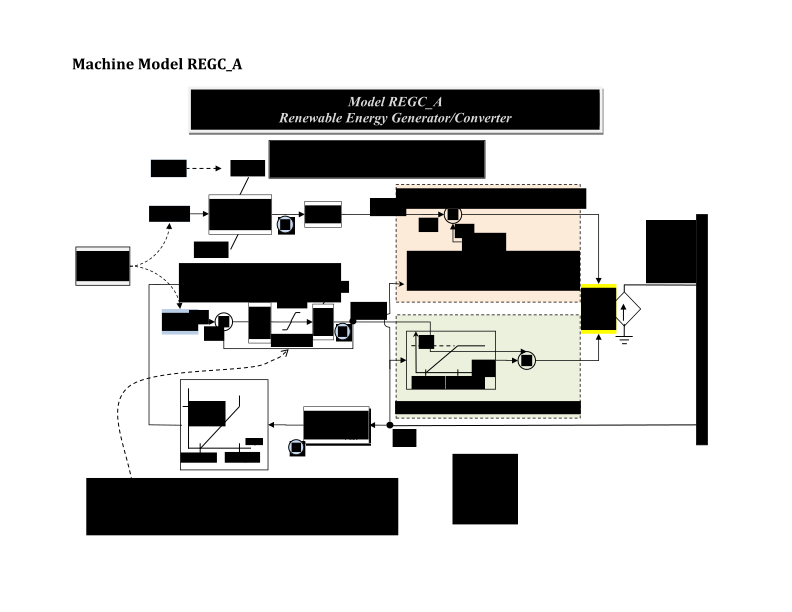
\includegraphics[width=\linewidth]{plots/gfl_diagram.png}
        \caption{GFL control diagram \cite{diagram:gfl}.}
        \label{fig:control_gfl}
    \end{subfigure}
    \hfill
    \begin{subfigure}[t]{0.52\textwidth}
        \centering
        \includegraphics[width=\linewidth]{plots/gfm_diagram.png}
        \caption{GFM control diagram \cite{diagram:gfm}.}
        \label{fig:colmena_gfm}
    \end{subfigure}
    \caption{Different control diagram of the converter.}
    \label{fig:gflgfm}
\end{figure}


\subsubsection*{Load Shedding Role}

This role is activated when the frequency is outside the admissible range, and the AGC role has been active on a nearby generator (or power-injecting converter) for at least 30 seconds. When activated, the agent linearly reduces the power consumed by its coupled load. When the role deactivates (e.g., frequency returns to the acceptable range), this load reduction is reversed.

\section{Prototype Implementation}

\subsection*{Service Description}

The prototype simulates an electrical grid subject to multiple perturbations occurring over the simulation period. The objective of the COLMENA service is to maintain the grid frequency within an acceptable range, defined as $[\omega_{\min}, \omega_{\max}] = [0.9999, 1.0001]$ p.u. (per unit). The KPI associated with the frequency metric ($\omega$) triggers the activation of the GFM Activation and AGC roles. The primary goal is to demonstrate that the activation of these roles effectively corrects frequency deviations.

The prototype deploys four agents, each within a separate Docker container. Two agents are paired with converters (initially operating in GFL mode), and the other two are paired with generators (or generator-like devices). The roles associated with the converters allow changing their control mode from GFL to GFM, while the AGC role dynamically adjusts the power output of the generators/converters using a PI controller.

\subsection{ANDES Interaction}

Grid simulation is performed using the ANDES package. The grid is initialized with values from a pre-calculated power flow solution. After initialization, ANDES is deployed as a service accessible via a Flask interface, listening on a specific port. Agents interact with ANDES by sending HTTP requests to query device data or modify parameters. Changing grid parameters follows a similar request-response procedure. At any point during the simulation, agents can send requests to modify grid parameters (e.g., set points, device status). These requests are received by the Flask application and reflected immediately in the ANDES simulation state. Since the ANDES simulation and the COLMENA agents operate with synchronized clocks (running in parallel), changes requested by COLMENA are applied at the correct simulation time in ANDES.

\begin{algorithm}
    \caption{High-Level Simulation Loop with COLMENA-ANDES Interaction}
    \label{algo:COLMENAANDES}
    \begin{algorithmic}[1]
        \State Initialize grid states $x$ to $x_0$ using Power Flow results.
        \For{each agent in Agents}
            \For{each device in controllable\_devices}
                \If{device is not currently controlled}
                    \State Pair agent with device
                    \State Mark device as controlled
                \EndIf
            \EndFor
        \EndFor
        \While{simulation time $<$ T\_{final}}
            \State Agents check KPIs based on latest data.
            \State Agents activate/execute roles based on KPIs.
            \State Roles send parameter change requests to ANDES via Flask.
            \State Roles request updated simulation data from ANDES via Flask.
            \State ANDES receives parameter changes via Flask.
            \State ANDES advances simulation by $\Delta t$ (e.g., 0.1s).
            \State ANDES provides updated state data upon request.
        \EndWhile
        \State Finalize simulation and collect results.
    \end{algorithmic}
\end{algorithm}

\begin{figure}[h]
    \centering
    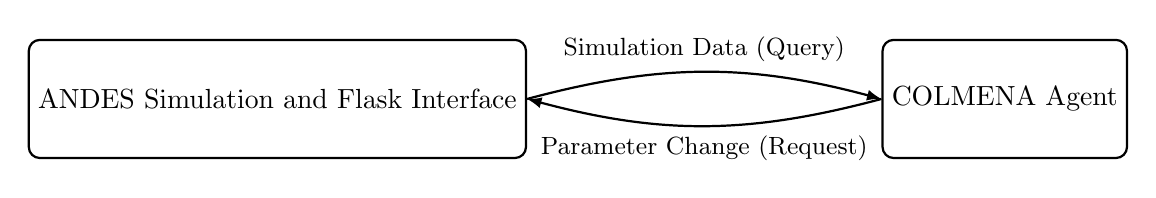
\begin{tikzpicture}[node distance=9cm and 4.5cm, >=latex, thick]
        % Define smaller nodes with rounded corners
        \node[draw, rectangle, rounded corners, minimum width=3.1cm, minimum height=1.5cm, align=center] (sim) {ANDES Simulation and Flask Interface};
        \node[draw, rectangle, rounded corners, minimum width=3.1cm, minimum height=1.5cm, align=center, right=of sim] (agent) {COLMENA Agent};

        % Adjusted rounded arrows with different start and end positions
        \draw[->, rounded corners] (sim.east) to[out=15, in=165] node[above, font=\small] {Simulation Data (Query)} (agent.west);
        \draw[<-, rounded corners] (sim.east) to[out=-15, in=-165] node[below, font=\small] {Parameter Change (Request)} (agent.west);
    \end{tikzpicture}
    \caption{Data flow between the ANDES Simulation (via Flask) and a COLMENA Agent.}
    \label{fig:sim_agent_interaction}
\end{figure}

In the current implementation, agents exclusively receive data from and send commands to their directly paired device. This constraint stems from the one-to-one agent-device pairing defined for this prototype.

\subsection{Simulation Setup}

The simulation starts from a pre-computed steady-state power flow solution. To introduce dynamic behavior, several disturbances are manually triggered during the simulation. These disturbances include step changes in load, representing consumption variability, and a transmission line outage. These events perturb the grid state, prompting responses from the COLMENA agents. The goal is to demonstrate the actions taken by the agents to maintain grid frequency stability in response to these disturbances. The simulation runs for 55 seconds. We compare the transient frequency response to a control simulation where no COLMENA agent roles are active.

\begin{table}[h]
    \centering
    \begin{tabular}{|l|l|l|}
    \hline
    \textbf{Perturbation} & \textbf{Device/Element} & \textbf{Change Details} \\
    \hline
    Line Outage & Line 2 & Disconnected at $t = 3\,$s \\
    Load Increase & Load 1 & Power demand increases by 50\% at $t = 18\,$s \\
    Load Increase & Load 2 & Power demand increases by 50\% at $t = 33\,$s \\
    \hline
    \end{tabular}
    \caption{Scheduled Grid Disturbances}
    \label{tab:disturbances}
\end{table}

\subsection{Results}

To evaluate the performance, we compare the results against a control simulation using the identical grid model and disturbance sequence, but without any COLMENA agent roles activated. The evolution of key metrics, particularly grid frequency, is compared between the two simulations.

\begin{figure}[h!]
    \centering
    \begin{subfigure}[t]{0.60\textwidth}
        \centering
        \includegraphics[width=\linewidth]{plots/control_omega2.png}
        \caption{Frequency ($\omega$) evolution (Control Case).}
        \label{fig:control_omega}
    \end{subfigure}
    \hfill
    \begin{subfigure}[t]{0.65\textwidth}
        \centering
        \includegraphics[width=\linewidth]{plots/genrou_omega.png}
        \caption{Frequency ($\omega$) evolution (COLMENA Case).}
        \label{fig:colmena_omega}
    \end{subfigure}
    \caption{Comparison of grid frequency ($\omega$ in p.u.) evolution in control and COLMENA-managed simulations.}
    \label{fig:omega_comparison}
\end{figure}

As shown in Figure \ref{fig:omega_comparison}, the grid frequency ($\omega$) in the COLMENA-controlled simulation demonstrates improved stability and faster recovery towards the nominal value (1 p.u.) following disturbances, compared to the control case. This improvement is attributed to the timely activation and actions of the defined roles (AGC and GFM Activation).

\begin{figure}[h!]
    \centering
    
    % Plot 1: Monitoring Role
    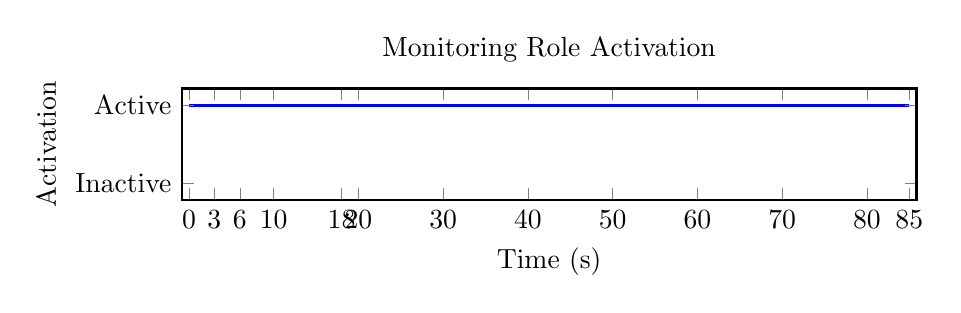
\begin{tikzpicture}
    \begin{axis}[
        width=0.9\linewidth,
        height=3cm,
        xlabel={Time (s)},
        ylabel={Activation},
        ymin=-0.2, ymax=1.2,
        xmin=0, xmax= 85,
        xtick={0, 3, 6, 10, 18, 20, 30, 40, 50, 60, 70, 80, 85},,
        ytick={0,1},
        yticklabels={Inactive, Active},
        title={Monitoring Role Activation},
        enlargelimits=0.01,
        axis on top,
        thick
    ]
    \addplot [
        const plot,
        draw=blue,
        line width=1pt
    ] coordinates {
        (0,1) (85,1)
    };
    \end{axis}
    \end{tikzpicture}
    
    \vspace{0.5cm}
    
    % Plot 2: AGC Role
    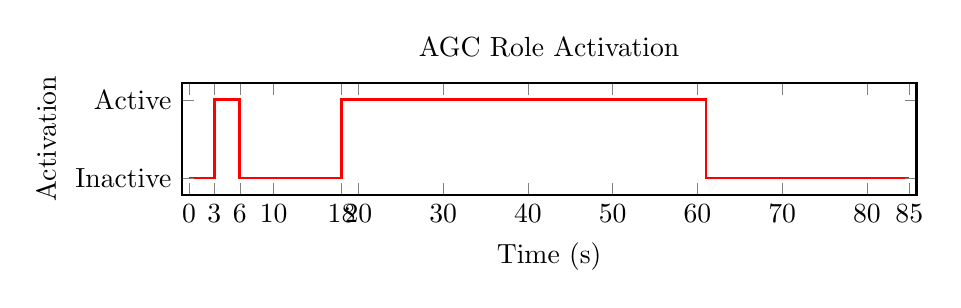
\begin{tikzpicture}
    \begin{axis}[
         width=0.9\linewidth,
        height=3cm,
        xlabel={Time (s)},
        ylabel={Activation},
        ymin=-0.2, ymax=1.2,
        xmin=0, xmax=85,
        xtick={0, 3, 6, 10, 18, 20, 30, 40, 50, 60, 70, 80, 85},
        ytick={0,1},
        yticklabels={Inactive, Active},
        title={AGC Role Activation},
        enlargelimits=0.01,
        axis on top,
        thick
    ]
    \addplot [
        const plot,
        draw=red,
        line width=1pt
    ] coordinates {
        (0,0) (3,0) (3,1) (6,1) (6,0) (18,0) (18,1) (61,1) (61,0) (85,0)
    };
    \end{axis}
    \end{tikzpicture}
    
    \vspace{0.5cm}
    
    % Plot 3: GFM Activation Role
    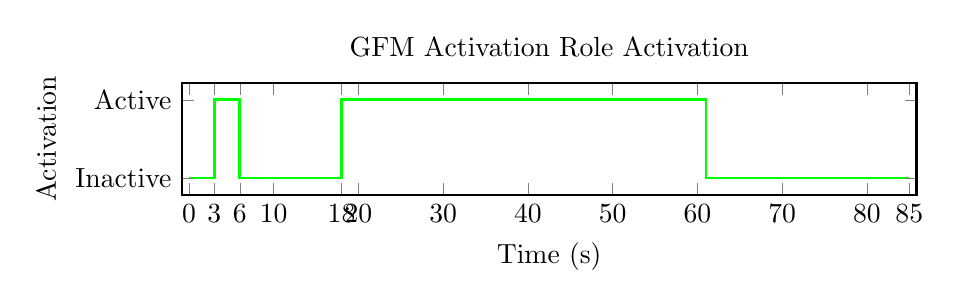
\begin{tikzpicture}
    \begin{axis}[
         width=0.9\linewidth,
        height=3cm,
        xlabel={Time (s)},
        ylabel={Activation},
        ymin=-0.2, ymax=1.2,
        xmin=0, xmax=85,
        xtick={0, 3, 6, 10, 18, 20, 30, 40, 50, 60, 70, 80, 85},
        ytick={0,1},
        yticklabels={Inactive, Active},
        title={GFM Activation Role Activation},
        enlargelimits=0.01,
        axis on top,
        thick
    ]
    \addplot [
        const plot,
        draw=green,
        line width=1pt
    ] coordinates {
        (0,0) (3,0) (3,1) (6,1) (6,0) (18,0) (18,1) (61,1) (61,0) (85,0)
    };
    \end{axis}
    \end{tikzpicture}
    
    \caption{Activation status (1=Active, 0=Inactive) of key roles during the COLMENA simulation, triggered by frequency deviations following disturbances at t=3s, t=18s, and t=33s.}
    \label{fig:activation_plots}
\end{figure}
    
Furthermore, Figure \ref{fig:activation_plots} illustrates that the AGC and GFM Activation roles activate appropriately in response to frequency deviations caused by the grid disturbances initiated at t=3s, t=18s, and t=33s and deactivate when the metric is back to its nominal value. In the simulation we see that after the action of the roles on the grid this one goes back to a steady state condition which is what we expected. Additionally, the action of the four agents on 2 generators and 2 converters changed the behavior of the whole grid. 

\section{Milestone Review}

\subsection*{Milestone 1: Initial Prototype and Validation}

This prototype integrates the initial implementation of algorithms developed within the project. The applicability of the COLMENA technology is validated in a pilot simulation setup. The analysis involves dynamic power system simulations, which require modeling not only the magnitudes controlled by devices (like power converters) but also the control loops themselves. For instance, the roles controlling generator power output directly influence the system's dynamic behavior. To this end, the prototype includes initial heuristics enabling transitions between converter operating modes (e.g., GFL to GFM). The completion of this milestone confirms that an initial version of the prototype is operational and capable of executing this type of flexible control logic.

\subsection*{Milestone 2: Open-Source Publication}

Following internal validation, this milestone involved publishing the initial pilot version in an open-access repository (GitHub/GitLab) \cite{git:eroots}. The purpose is to facilitate transparency, community engagement, and external testing. The codebase relies on open-source Python packages for power system analysis, primarily ANDES \cite{article:andes}. ANDES is licensed under the GPLv3, a copyleft license permitting modification and redistribution under the same terms. The publication of the repository fulfills the objectives of this milestone.

\section{Conclusion}

This prototype represents an initial step towards developing a comprehensive test case for applying COLMENA in power grid control. The results demonstrate that roles activate appropriately in response to KPI violations, guiding the system back towards desired operating states (Figure \ref{fig:omega_comparison}). This corrective behavior is achieved through the grid modifications executed by the roles (Figure \ref{fig:activation_plots}). Compared to the control simulation, the COLMENA-controlled prototype exhibits fewer and shorter frequency KPI violations.

Future work involves leveraging upcoming COLMENA features for more precise metric and KPI handling. This includes defining KPIs more specific to individual roles and potentially incorporating geographical or topological scope. For instance, defining area-specific KPIs could ensure only relevant agents activate roles in response to local issues. Similarly, implementing more sophisticated rules for coordinating role activation, possibly combining operational KPIs with economic considerations, could enhance overall performance.

Additionally, anticipated COLMENA enhancements will facilitate inter-role communication. This capability will enable more complex, coordinated control strategies. We envision, for example, roles managing specific grid areas that communicate data to implement distributed Model Predictive Control (MPC) schemes. 
\nocite{*}
\printbibliography
\end{document}